% !TeX root = main.tex

\chapter{UNITS, PHYSICAL QUANTITIES, AND VECTORS}
\label{chap:units}
\includegraphics[width=\linewidth]{ch1title.png}\\

Physics is one of the most fundamental of the sciences. Scientists of all disciplines use the ideas of physics, including chemists who study the structure of molecules, palaeontologists who try to reconstruct how dinosaurs walked, and climatologists who study how human activities affect the atmosphere and oceans. Physics is also the foundation of all engineering and technology. No engineer could design a flat-screen TV, a prosthetic leg, or even a toaster for that matter without first understanding the basic laws of physics.

The study of physics is also an adventure. You’ll find it challenging, sometimes frustrating, occasionally painful, and often richly rewarding. If you’ve ever wondered why the sky is blue, how radio waves can travel through empty space, or how a satellite stays in orbit, you can find the answers by using fundamental physics. You’ll come to see physics as a towering achievement of the human intellect in its quest to understand our world and ourselves.

We’ll discuss the nature of physical theory and the use of idealized models to represent physical systems. We’ll introduce the systems of units used to describe physical quantities and discuss ways to describe the accuracy of a number. We’ll look at examples of problems for which we can’t (or don’t want to) find a precise answer, but for which rough estimates can be useful and interesting. Finally, we’ll study several aspects of vectors and vector algebra. We’ll need vectors throughout our study of physics to help us describe and analyze physical quantities, such as velocity and force, that have direction as well as magnitude.

\section{The Nature of Physics}
Physics is an \textit{experimental} science. Physicists observe the phenomena of nature and try to find patterns that relate these phenomena. These patterns are called physical theories or, when they are very well established and widely used, physical laws or principles.

\textit{A theory is not just a random thought or an unproven concept. Rather, a theory is an explanation of natural phenomena based on observation and accepted fundamental principles. An example is the well-established theory of biological evolution, which is the result of extensive research and observation by generations of biologists.}
\FloatBarrier
\begin{figure}[!h]
  \centering
  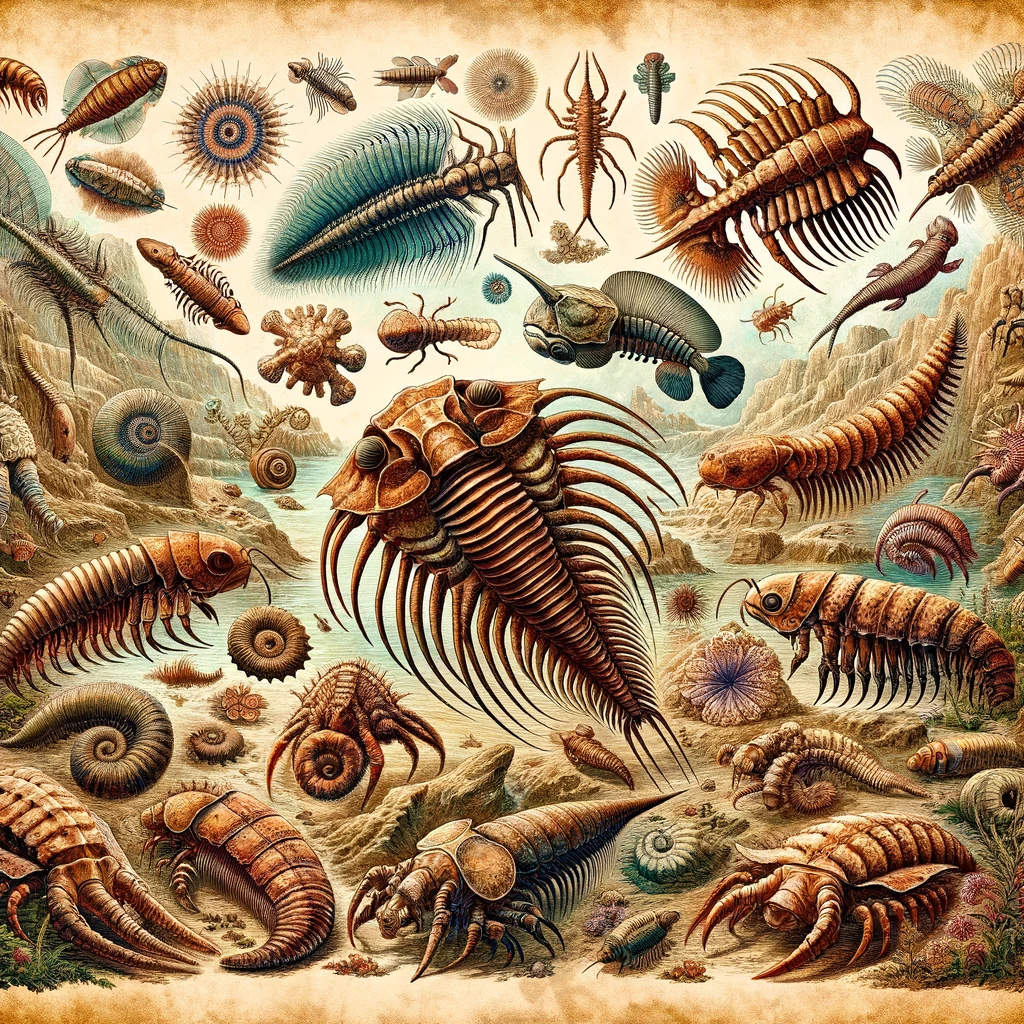
\includegraphics[width=0.4\linewidth]{ch1img0.png}
  \caption{Around 530 million years ago, a wide variety of animals burst onto the evolutionary scene in an event known as the Cambrian explosion.}
  \label{fig:ch1img0}
  \medskip
  \centering
  
\includegraphics[width=0.4\linewidth]{ch1img10.png}
  \caption{The Big Bang event is a physical theory that describes how the universe expanded from an initial state of high density and temperature.}
  \label{fig:ch1img10}
  \bigskip
\end{figure}
\FloatBarrier

To develop a physical theory, a physicist has to \textit{ask appropriate questions, design experiments to try and answer the questions, and draw appropriate conclusions} from the results. Legend has it that \textbf{Galileo Galilei} (1564-1642) dropped light and heavy objects from the top of the Leaning Tower of Pisa to find out whether their rates of fall were different. From examining the results, he deduced the theory that the acceleration of a freely falling object is independent of its weight. The development of physical theories such as Galileo's often takes an indirect path with blind alleys, wrong guesses and the discarding of unsuccessful theories in favour of more promising ones. Physics is not simply a collection of facts and principles; it is also the process by which we arrive at general principles that describe how the physical universe behaves.

No theory is ever regarded as the ultimate truth. It's always possible that new observations will require that a theory be revised or even discarded. We can disprove a theory by finding behaviour that is inconsistent with it, but we can never prove that a theory is always correct.
Galileo wasn't wrong! His theory was simply \textit{incomplete}. If we dropped the feather and the cannonball in a vacuum to eliminate the effects of air, then they \textbf{do fall at the same rate}. This theory has a range of validity: It only applies to objects for which the force exerted by the air is much less than the weight. Objects like feathers or parachutes are clearly outside this range.

\begin{figure}[htbp]
  \centering
  
\includegraphics[width=0.4\linewidth]{ch1img4.png}
  \caption{Newton's famed discovery of gravity.}
  \label{fig:ch1img4}
\end{figure}
%\FloatBarrier
\section{Solving Physics Problems}
We can attempt to solve physics problems with this robust strategy.

\begin{enumerate}
	\item \textbf{IDENTIFY} the relevant concepts:
	\begin{itemize}
		\item Use the physical conditions stated in the problem to help ascertain potentially useful concepts.
		\item Identify the target variables of the problem.
		\item Identify the known (and required) quantities, extremely important.
	\end{itemize}
	
	\item \textbf{SETUP} the problem:
	\begin{itemize}
		\item Given the gathered data, decide on the correct equations.
		\item Make sure that the variables correctly correlate to the equations.
	\end{itemize}

	\item \textbf{EXECUTE} the solution:
	\begin{itemize}
		\item Carefully evaluate the mathematics.
	\end{itemize}

	\item \textbf{EVALUATE} the answer:
	\begin{itemize}
		\item Sanity checks to eliminate common errors.
	\end{itemize}
\end{enumerate}

\bigskip

\textbf{Idealized Models}

In physics, a model is a simplified version of a physical system that would be too complicated to analyse in full detail. Lets look at an example.

Suppose we want to analyse the motion of a thrown baseball. How complicated is this problem? The ball is not a perfect sphere (raised seams), and it spins and moves through the air. Air resistance and wind influence its motion, the ball's weight varies a little as its altitude changes, and so on. If we try to include all these effects, the analysis gets hopelessly complicated. 

\begin{figure}[htbp]
  \centering
  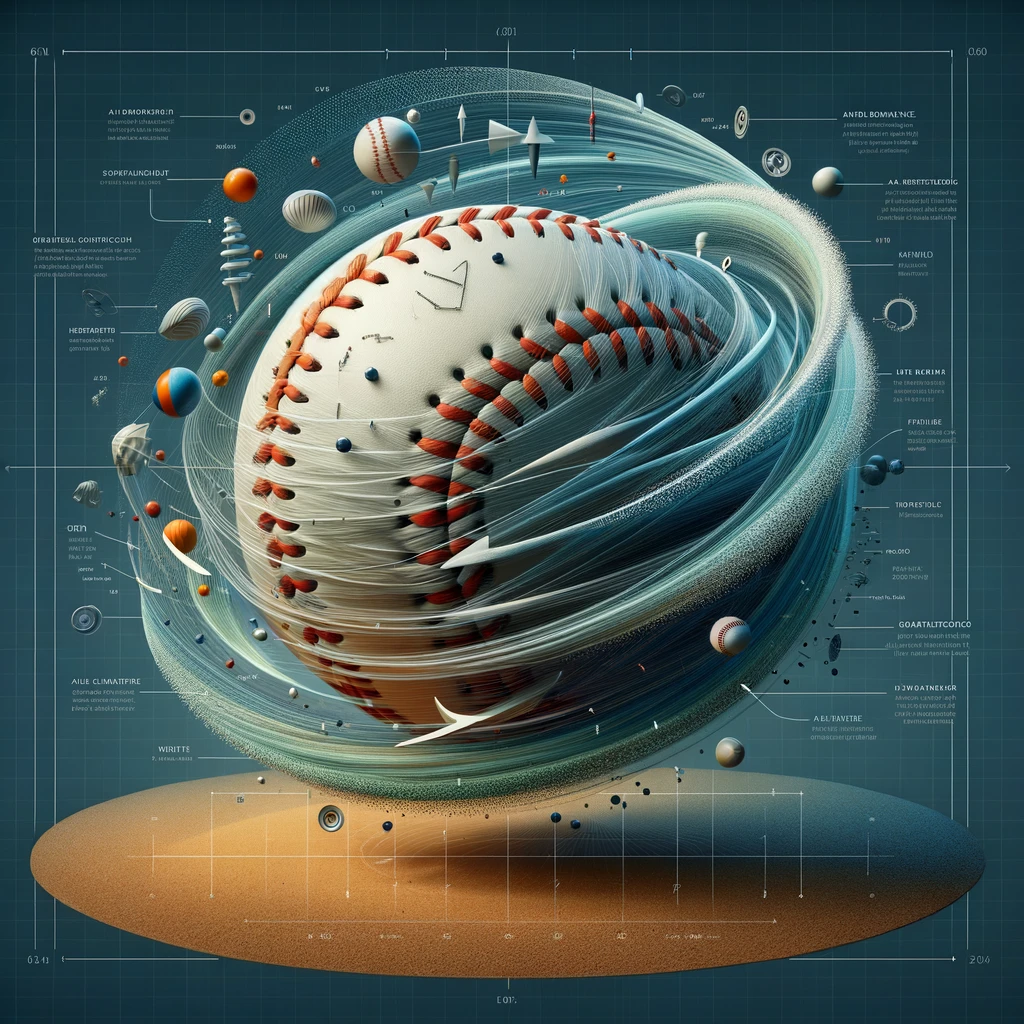
\includegraphics[width=0.4\linewidth]{ch1img5.png}
  \caption{Modelling the simplest of physical phenomena is often complex and necessitates idealized models.}
  \label{fig:ch1img5}
\end{figure}

Instead, we invent a simplified version of the problem. We ignore the size, shape, and rotation of the ball by representing it as a point object (or a particle). Similarly, we ignore air-resistance by making the ball move in a vacuum, and make the weight constant. Now we have a problem that is simple enough to deal with. We may overlook some subtle physical phenomenon while creating an ideal model, but we must be careful to not discard principal affects. For e.g, if we completely ignore gravitational effects, then our model makes an absurd prediction that when we throw the ball up, it will keep going up in a straight line with nothing to pull it back down, disappearing into space. \textbf{A useful model simplifies a problem enough to make it manageable, yet keeps its essential features.}

\begin{figure}[htbp]
 \centering
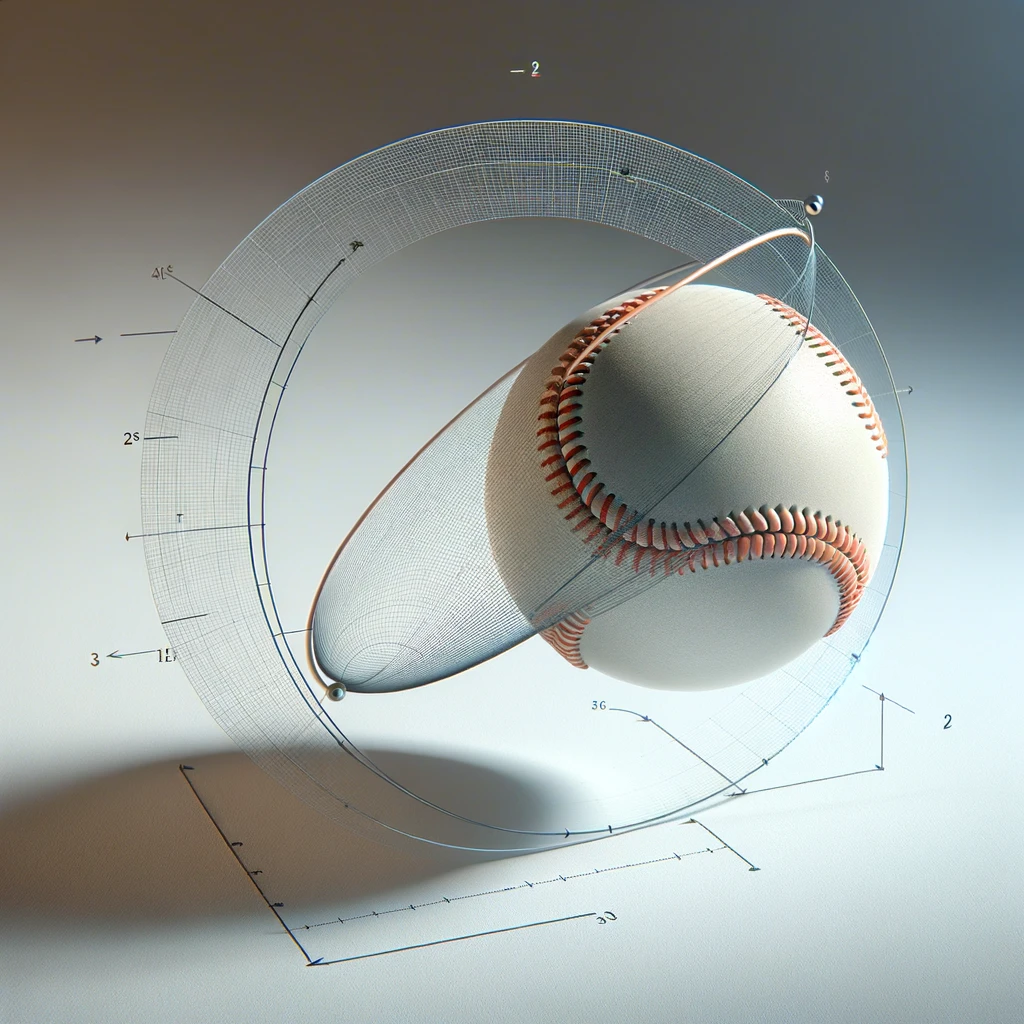
\includegraphics[width=0.4\linewidth]{ch1img6.png}
  \caption{A possible idealized model for analysing the motion of a thrown ball.}
  \label{fig:ch1img6}
\end{figure}

The validity of the predictions we make using a model is limited by the validity of the model itself. For e.g, Galileo's prediction about falling objects corresponds to an idealized model that does not include the effects of air resistance. The model works fairly well for a cannonball, but not so well for a feather.

\section{Standards and Units}
As we well know, physics is an experimental science. Experiments require measurements, and we generally use numbers to describe the results of measurements. Any number that is used to describe a physical phenomenon quantitatively is called a \textbf{physical quantity}. For example, two physical quantities that describe us are our weight and height. Some physical quantities are so fundamental that we can define them only by describing how to measure them. Such a definition is called an operational definition. Two examples are measuring a distance by using a ruler and measuring a time interval by using a stopwatch. In other cases, we define a physical quantity by describing how to calculate it from other quantities that we \textit{can} measure. Thus we might define the average speed of a moving object as the distance traveled (measured with a ruler) divided by the time of travel (measured with the stopwatch).

When we measure a quantity, we always compare it with some reference standard. When we say that a basketball hoop is 3.05 meters over the ground, we mean that this stick is 3.05 times as long as a meter stick, which we define to be 1 meter long. Such a standard defines a \textbf{unit} of the quantity. The meter is a unit of distance, and the second is a unit of time. When we use a number to describe a physical quantity, we must specify the unit that we are using; to describe a distance as simply "3.05" wouldn't mean anything meaningful. 

To make accurate, reliable measurements, we need units of measurement that do not change and can be duplicated by observers in various locations. The system of units used by scientists and engineers around the world is commonly called "the metric system", but since the 1950 it has been officially known as the \textbf{International System, or SI}.

\textbf{Time}

From 1889 until 1967, the unit of time was defined as a certain fraction of the mean solar day, the average time between successive arrivals of the sun at its highest point in the sky.
The present standard, adopted in 1967, is much more precise. It is based on an atomic clock, which uses the energy difference between the two lowest energy states of the Caesium atom (133Cs). When bombarded by microwaves of precisely the proper frequency, Caesium atoms undergo a transition from one of these states to the other. One second (abbreviated s) is defined as the time required for 9,192,631,770 cycles of this microwave radiation.

\begin{figure}[htbp]
	\centering
	
\includegraphics[width=0.4\linewidth]{ch1img7.png}
	\caption{Measuring the second as a difference between the two lowest energy states of the Caesium atom.}
	\end{figure}

\medskip

\textbf{Length}

In 1960 an atomic standard for the meter was also established, using the wavelength of the orange-red light emitted by excited atoms of krypton 186Kr2. From this length standard, the speed of light in vacuum was measured to be 299,792,458 m/s. In November 1983, the length standard was changed again so that the speed of light in vacuum was defined to be precisely 299,792,458 m/s. Hence the new definition of the meter (abbreviated m) is the distance that light travels in vacuum in 1/299,792,458 a second. This modern definition provides a much more precise standard of length than the one based on a wavelength of light.

\begin{figure}[htbp]
  \centering
  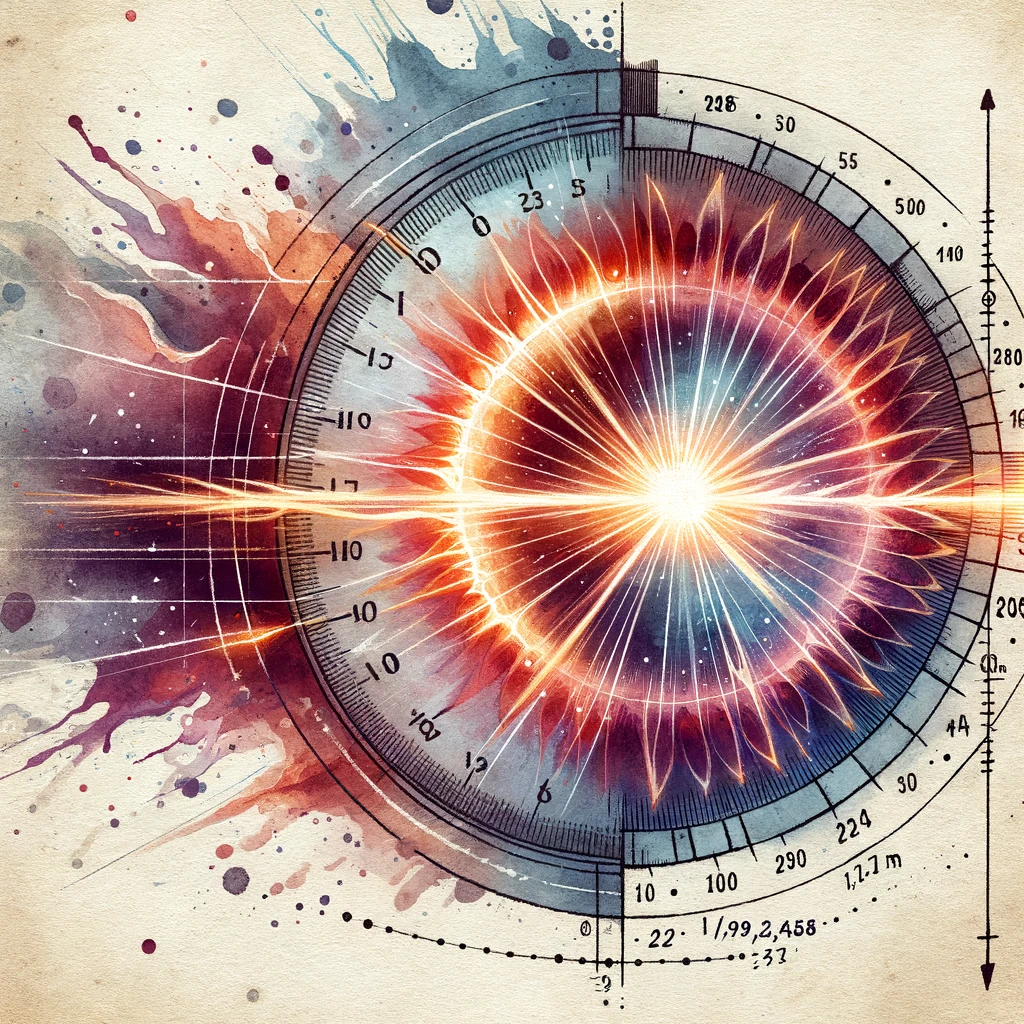
\includegraphics[width=0.4\linewidth]{ch1img8.png}
  \caption{Measuring the second as the time light takes to travel in vacuum in 1/299,792,458 s.}
  \label{fig:ch1img8}
\end{figure}

\textbf{Mass}

Until recently the unit of mass, the kilogram (abbreviated kg), was defined to be the mass of a metal cylinder kept at the International Bureau of Weights and Measures in France. This was a very inconvenient standard to use. Since 2018 the value of the kilogram has been based on a fundamental constant of nature called Planck’s constant (symbol h), whose defined value $h = 6.62607015 \times 10^{-34}\, \text{kg}\cdot\text{m}^{2}/ \, \text{s}$ is related to those of the kilogram, meter, and second.
 
Given the values of the meter and the second, the masses of objects can be experimentally determined in terms of h. The gram (which is not a fundamental unit) is 0.001 kilogram. Other derived units can be formed from the fundamental units. For example, the units of speed are meters per second, or m>s; these are the units of length (m) divided by the units of time (s).

\section{Using and Converting Units}

We use equations to express relationships among physical quantities, represented by algebraic symbols. Each algebraic symbol always denotes both a number and a unit. For e.g., \textit{d} might represent a distance of 10 m, \textit{t} a time of 5 s, and \textit{v} a speed of 2 m/s.
\vspace{-20pt}

\begin{tipbox}
An equation must always be \textbf{dimensionally consistent.} You can't add apples and automobiles; two terms may be added or equated only if they have the same units. For e.g., if an object moving with constant speed \textit{v} travels a distance \textit{d} in a time \textit{t}, these quantities are related by the equation\\
\begin{center}
	$\textbf{\textit{{d = v t}}}$
\end{center}
\end{tipbox}
\vspace{-30pt}
If $d$ is measured in meters, then the product $v t$ must also be expressed in meters. Using the above, we can write
\vspace{-21pt}
\begin{mathbox}
\begin{center}
$10 m = \Biggl(2  \ \frac{m} {\cancel{s}} \Biggr)\ (5 \cancel{s}) $
\end{center}
\end{mathbox}
\vspace{-20pt}

\begin{examplebox}
\textbf{Example 1.1} \textit{Converting speed units.}\\

The world land speed record of 763.0 mi/h was set on October 15, 1997, by Andy Green in the jet-engine car "Thrust SSC". Express this speed in meters per second.
\begin{mathbox}
\begin{align*}
&= \left(763.0 \, \frac{\text{mi}}{\text{h}}\right) \\
&= 763 \, \frac{\text{\cancel{mi}}}{1 \, \text{\cancel{h}}} \times \frac{1 \, \text{\cancel{h}}}{3600 \, \text{sec}} \times \frac{1.609 \, \text{\cancel{km}}}{1 \, \text{\cancel{mi}}} \times \frac{1000 \, \text{m}}{1 \, \text{\cancel{km}}} \\ \\
&= \underline{341.01 \, \text{m/s}}
\end{align*}
\end{mathbox}
\end{examplebox}
\bigskip

\begin{examplebox}
\textbf{Example 1.2} \textit{Converting volume units.}\\

One of the world’s largest cut diamonds is the First Star of Africa (mounted in the British Royal Sceptre and kept in the Tower of
London). Its volume is 1.84 cubic inches. What is its volume in cubic centimeters? In cubic meters?
\begin{mathbox}
\begin{align*}
&= \left(1.84\, \text{in.}^3\right) \\
&= 1.84 \times 2.54 \, ^ 3 \; \left(\frac{\cancel{\text{in.}^3} \, \text{cm}^3} {\cancel{\text{in.}^3}} \right) \\
&= \underline{30.2 \, \text{cm}^3 \quad \langle\text{in cm$^3$}}\rangle \\ \\
&= \left(30.2 \, \text{cm}^3\right) \\
&= \left(30.2 \, \text{cm}^3\right) \times \left(\frac{1 \, \text{m}}{100 \, \text{cm}} \right) ^ 3 \\
&= \frac{30.2}{100^3} \, \left(\frac{\cancel{\text{cm}^3} \, \text{m}^3 }{\cancel{\text{cm}^3}} \right) \\
&= \underline{3.02 \times 10^{-5} \, \text{m}^3 \quad \langle\text{in m$^3$}}\rangle
\end{align*}
\end{mathbox}
\end{examplebox}

\section{Uncertainty and Significant Figures}
Measurements always have uncertainties. If we measure the thickness of the cover of a hardbound version of a book using an ordinary ruler, our measurement is reliable to only the nearest millimeter, and our result will be for e.g., $3$ mm. It would be \textit{wrong} to state this result as $3.00$ mm; given the limitations of the measuring device, we can't tell whether the actual thickness is $3.00$ mm or $3.25$ mm. But if we measure this with a micrometer caliper, a device that measures distances reliably to the nearest $0.01$ mm, the result will be $2.91$ mm. The distinction between the measurements with a ruler and with a caliper is in their \textbf{uncertainty}; the measurement with a caliper has a smaller uncertainty. This uncertainty is also called the error because it indicates the maximum difference there is likely to be between the measured value and the true value. The uncertainty of a measured value depends on the measurement technique (and equipment) used.

We often indicate the \textbf{accuracy} of a measured value, that is, how close it is likely to be to the true value, by writing the number, the symbol $\pm$, and a second number indicating the uncertainty of the measurement. If the diameter of a steel rod is given as $56.47 \pm 0.02$ mm, this means that the true value is likely to be within the range from $56.45$ mm to $56.49$ mm. In a commonly used shorthand notation, the number $1.654(21)$ means $1.654 \pm 0.0021$. The numbers in parentheses show the uncertainty in the final digits of the main number.

We can also express accuracy in terms of the maximum likely fractional error or percent error (also called fractional or percent uncertainty). A resistor labeled "$47$ ohms $\pm 10\%$" probably has a true resistance that differs from $47$ ohms by no more than $10$\% of $47$ ohms-that is, by about $5$ ohms. The resistance is probably between $42$ and $52$ ohms. 

In many cases, the uncertainty of a number is not stated explicitly. Instead, the uncertainty is indicated by the number of meaningful digits, or \textbf{significant figures}, in the measured value. We gave the thickness of the book as $2.91$ mm, which has three significant figures. By this we mean that the first two digits are known to be correct, while the third digit is uncertain. The last digit is in the hundredths place, so the uncertainty is about $0.01$ mm. Two values with the \textit{same} number of signifcant figures may have \textit{different} uncertainties; a distance given as $137$ km also has three significant figures, but the uncertainty is about $1$ km.

When we use numbers that have uncertainties to compute other numbers, the computed numbers are also uncertain. When numbers are multiplied or divided, the result can have no more significant figures than the factor with the fewest significant figures has. For e.g., $3.1416 \times 2.34 \times \textcolor{red}{\textit{0.58}} = 4.3$. When we add and subtract numbers, it's the location of the decimal point that matters, not the number of significant figures. For e.g., $123.62 + \textcolor{red}{\textit{8.9}} = 132.5$

\begin{tipbox}
About calculations that involve multiple steps: As we work, it's helpful to keep extra significant fgures in our calculations. Once we havethe final answer, we round it to the correct number of significant figures. This will lead to the most accurate results. 
\end{tipbox}

While working with very large or very small numbers, we can show significant figures much more easily by using \textbf{scientific notation}, sometimes called \textbf{powers-of-10 notation}. The distance from the earth to the moon is about $384,000,000$ m, but writing the number in this form doesn't indicate the number of significant features. Instead, we move the decimal point eight places to the left (corresponding to dividing by $10^8$) and multiply by $10^8$; that is\\
\begin{center}
$384,000,000$ m = $3.84 \times 10^8$ m
\end{center}

Finally, \textbf{precision} is not the same as \textit{accuracy}. A cheap digital watch that gives the time as 10:35:17 a.m. is very precise (time given to the second, if not better), but if the watch runs several minutes slow, then this value isn't quite \textit{accurate}. On the other hand, a grandfather clock might be quite accurate (that is, display the correct time), but it may not be as precise if it simply does not show the second hand. A high quality measurement is both \textbf{precise} and \textbf{accurate}.

\begin{examplebox}
\textbf{Example 1.3} \textit{Significant figures in multiplication.}\\

The rest energy $E$ of an object with rest mass $m$ is given by Albert Einstein's famous equation $E = mc^2$, where $c$ is the speed of light in vacuum. Find $E$ for an electron for which (to three significant figures) $m = 9.11 \times 10^{-31}$ kg. The SI unit for $E$ is the joule (J); $1 \text{J} = 1 \text{kg} \cdot \text{m}^2 / \text{s}^2$.
\bigskip
\begin{mathbox}
\begin{align*}
&= \left(9.11 \times 10^{-31} \, \text{kg}\right) \, \left(2.99792458 \times 10^{8} \, \text{m/s}\right)^{2} \\
&= \left(9.11\right)\left(2.99792458\right)^2 \left(10^{-31}\right) \left(10^8\right)^2 \text{kg} \cdot \text{m}^2\text{/}\text{s}^2 \\
&= \left(81.876596782924087004\right) \, \left(10\right)^{-31 + \left(2 \times 8\right)} \text{kg} \cdot \text{m}^2\text{/}\text{s}^2 \\
&= \left(81.876596782924087004\right) \, \left(10\right)^{-15} \text{kg} \cdot \text{m}^2\text{/}\text{s}^2 \\ \\
&= \underline{8.19 \times \left(10\right)^{-14} \text{J}}
\end{align*}
\end{mathbox}
\end{examplebox}

\section{Estimates and Orders of Magnitude}
We have stressed the importance of knowing the accuracy of numbers that represent physical quantities. But even a very crude estimate of a quantity often gives us useful information. Sometimes we know how to calculate a certain quantity, but we have to guess at the data we need for the calculation. Or the calculation might be too complicated to carry out exactly, so we make rough approximations. In either case, our result is also a guess, but such a guess can be useful even if it is uncertain by a factor of two, ten, or more. Such calculations are called \textbf{order-of-magnitude estimates}. The great Italian-American nuclear physicist Enrico Fermi (1901-1954) called them "back-of-the-envelope calculations".

\begin{examplebox}
 \textbf{Example 1.4} \textit{An order-of-magnitude estimate.}\\

You are writing an adventure novel in which the hero escapes with a billion dollars’ worth of gold in his suitcase. Could anyone carry that much gold? Would it fit in a suitcase?
\bigskip
\begin{mathbox}
\begin{align*}
\text{Price of Gold per kilo: } \$62,467 / \,\text{kg}\\
\text{\$1 Billion: } 1,000,000,000 \\
\text{The weight of the suitcase to enable carrying \$1 Billion: } 1,000,000,000 / 62,467 \\ 
=16,008 \,\text{kg}
\end{align*}
\end{mathbox}
It would be close to impossible for a typical suitcase to carry \approx 16,000 kg of gold.
\end{examplebox}

\section{Vectors and Vector Addition}
Some physical quantities, such as time, temperature, mass, and density, can be described completely by a single number with a unit. But many other important quantities in physics have a \textit{direction} associated with them and cannot be described by a single number. A simple example is the motion of an airplane: We must not only say how fast the plane is moving but also the direction it's moving in. The speed of the airplane combined with its direction of motion constitute a quantity called \textit{velocity}. Another example is \textit{force}, which in physics means the push or pull exerted on an object. 
Giving a complete description of a force means describing both how hard the force pushes or pulls on the object and the direction of push or pull. When a physical quantity is described by a single number, we call it a \textbf{scalar quantity}. In contrast, a \textbf{vector quantity} has both a \textit{magnitude} and a \textit{direction} in space. Calculations with vectors require a different set of operations relative to the scalar quantities we usually work with.

\begin{infobox}
    \begin{center}
        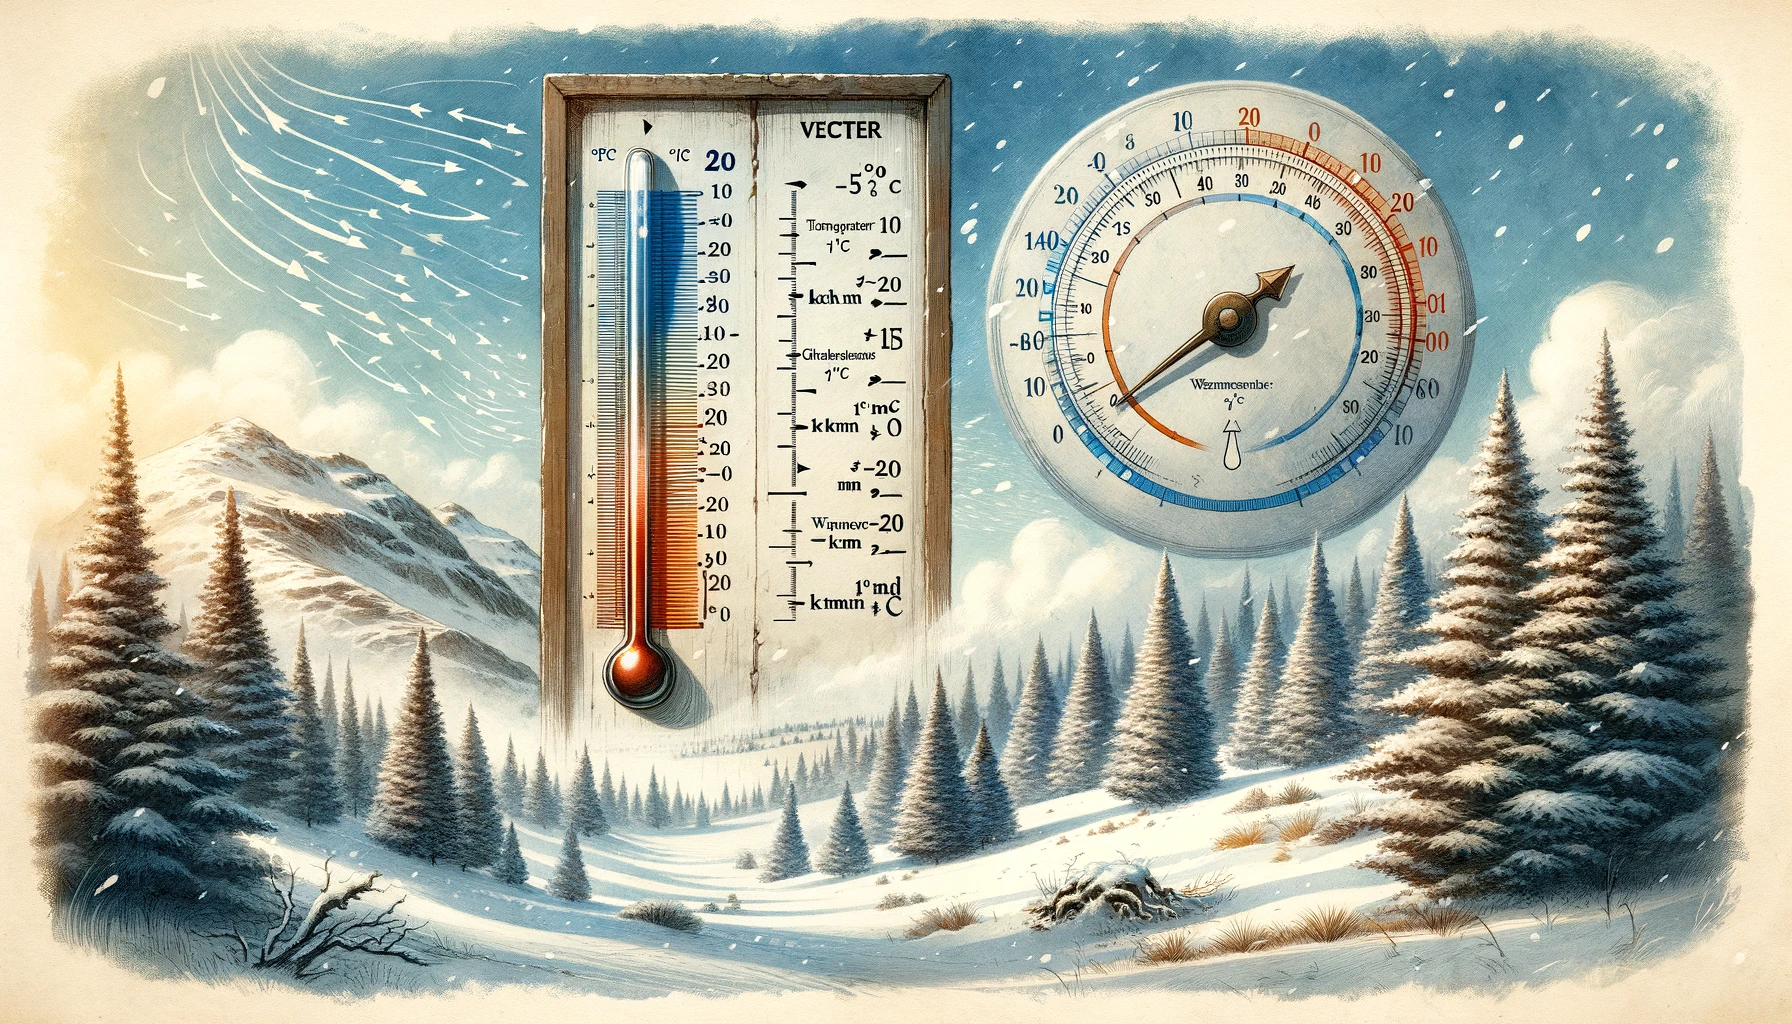
\includegraphics[width=\linewidth]{ch1img11.png}
    \end{center}
Scalar Temperature, Vector Wind: The comfort level on a wintry day depends on the temperature, a scalar quantity that can be positive or negative (say, +5$^{\circ}$C or -20$^{\circ}$C) but has no direction. It also depends on the wind velocity, a vector quantity with both magnitude and direction (for example, 15 km>h from the west).
\end{infobox}

To understand vectors better, we can start by looking at the simplest vector quantity, \textbf{displacement}, which is the change in the position of an object. Displacement is a vector quantity because we must state not only how far the object moves but also in what direction. Walking 3 km north, and walking 3 km south lead to different places. While they have the same magnitude, they have different directions. 
\begin{itemize}
\item We represent displacement by an arrow with a starting and ending position, pointing in a particular direction.
\item A displacement is always a straight arrow directed from the starting position to the ending position. It does not depend on the path taken, even if the path is curved.
\item Total displacement for a round trip is 0, regardless of the path taken or distance traveled.
\end{itemize}

If two vectors have the same direction, they are \textbf{parallel}. If they have the same magnitude and the same direction, they are \textit{equal}, no matter where they are located in space. The negative of a vector would be the same vector in magnitude, but points in the opposite direction, also called \textbf{antiparallel}.

\begin{tipbox}
\begin{itemize}
\item We denote a vector notationally as : $\overrightarrow{A}$.
\item We denote magnitude of a vector either as A without the arrow, or $\left | \overrightarrow{A} \right |$
\item The magnitude of a vector quantity is a scalar quantity (a number) and is \textit{always positive}.
\item Vectors and Scalars are \textit{different} quantities.
\end{itemize}
\end{tipbox}

\subsection*{Vector Addition and Subtraction}
Suppose a particle undergoes a displacement $\overrightarrow{A}$ followed by a second displacement $\overrightarrow{B}$. The final result is the same as if the particle had started at the same initial point and undergone a single displacement $\overrightarrow{C}$. We call displacement $\overrightarrow{C}$ the \textbf{vector sum}, or \textbf{resultant}, of displacements $\overrightarrow{A}$ and $\overrightarrow{B}$. We express this relationship symbolically as\\

\begin{center}
$\overrightarrow{C} = \overrightarrow{A} + \overrightarrow{B}$
\end{center}

\begin{figure}[htbp]
 \centering
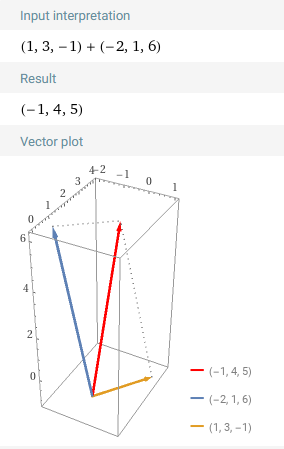
\includegraphics[width=0.5\linewidth]{ch1img13.png}
  \caption{Vector addition.}
  \label{fig:ch1img13}
\end{figure}

We can \textit{subtract} vectors as well as add them. We can define the difference $\overrightarrow{A} - \overrightarrow{B}$ to be the vector sum of $\overrightarrow{A}$ and $-\overrightarrow{B}$:\newline

\begin{center}
$\overrightarrow{A} - \overrightarrow{B} = \overrightarrow{A} + \left(- \overrightarrow{B}\right)$
\end{center}

\begin{examplebox}
\textbf{Example 1.5} \textit{Adding two vectors at right angles.}\\

A cross-country skier skis 1.00 km north and then 2.00 km east on a horizontal snowfield. How far and in what direction is she from the starting point?
\begin{center}
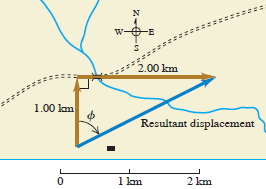
\includegraphics[width=0.5\linewidth]{ch1img14.png}
\end{center}
\begin{mathbox}
\begin{align*}
&= \sqrt{\left(1.00 \text{km}\right)^2 + \left(2.00 \text{km}\right)^2}\\
&\underline{\text{Resultant displacement} = 2.24 \text{km}}\\\\
\tan \phi &= \frac{2.00}{1.00} = 2.00\\
\phi &= \arctan 2.00\\
&= \underline{63.4 ^\circ\, \text{East of North}}
\end{align*}
\end{mathbox}
\end{examplebox}
\bigskip

\section{Components of Vectors}
Previously, we used the properties of right triangles to add vectors, but calculations with right triangles only work when the two vectors are perpendicular. We need a simple, more general method for adding vectors. This is called the methods of \textit{components}.

To define what we mean by the components of a vector $\overrightarrow{A}$, we begin with a rectangular (Cartesian) coordinate system of axes. If we think of $\overrightarrow{A}$ as a displacement vector, we can regard $\overrightarrow{A}$ as the sum of a displacement parallel to the x-axis and a displacement parallel to the y-axis. We use the numbers $A_x$ and $A_y$ to tell us how much displacement there is parallel to both $x$ and $y$ axis respectively.\\

We can calculate the components of $\overrightarrow{A}$  if we know its magnitude $A$ and its direction. We’ll describe the direction of a vector by its angle relative to some reference direction. In the figure above, this reference direction is the positive x-axis, and the angle between $\overrightarrow{A}$ and the positive x-axis is \theta \,  (the Greek letter theta). \\\\
Imagine that $\overrightarrow{A}$  originally lies along the positive x-axis and that you then rotate it to its true direction, as indicated by the arrow, on the arc for angle \theta. If this rotation is from the +x-axis toward the +y-axis, as is the case in the earlier figure, then u is positive; if the rotation is from the +x-axis toward the -y-axis, then \theta \, is negative. Thus the +y-axis is at an angle of $90^\circ$, the negative x-axis at $180^\circ$, and the negative y-axis at $270^\circ$ (or $-90^\circ$). If \theta \, is measured in this way, then from the definition of the trigonometric functions,

\begin{figure}[htbp]
 \centering
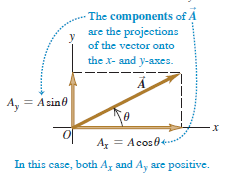
\includegraphics[width=0.3\linewidth]{ch1img15.png}
  \caption{Components of a vector.}
  \label{fig:ch1img15}
\end{figure}
\FloatBarrier

\textbf{Caution:} Relating a vector’s magnitude and direction to its components are correct only when the angle \theta\, is measured from the positive x-axis. If the angle of the vector is
given from a different reference direction or you use a different rotation direction, the relationships are different!

\begin{mathbox}
\begin{align*}
\frac{A_x}{A} = \cos \theta \qquad &\text{and} \qquad \frac{A_y}{A} = \sin \theta \\
A_x = A \cos \theta \qquad &\text{and} \qquad A_y = A \sin \theta \\
\end{align*}
\centerline{\textit{$\theta$ measured from the positive x-axis moving towards the positive y-axis.}}
\end{mathbox}

\begin{examplebox}
\textbf{Example 1.6} \textit{Finding components.}\\

(a) What are the x- and y-components of $\overrightarrow{D}$ in fig. a. The magnitude of the vector is $D$ = 3.00 m, and angle \alpha\, = $45^\circ$. (b) What are the x- and y-components of $\overrightarrow{E}$ in fig. b? The magnitude of the vector is $E$ = 4.50 m, and angle \beta \, = $37.0^\circ$.

\begin{center}
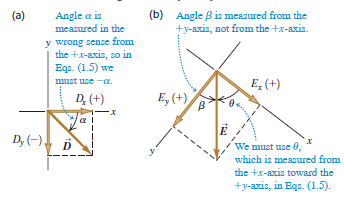
\includegraphics[width=0.5\linewidth]{ch1img16.png}
\end{center}
\begin{mathbox}
\begin{align*}
\text{For fig a,}\\
D_x &= D \, \cdot \cos \left(- \alpha\right)\\
&= 3.00 \text{m} \times \cos\left(-45^\circ\right)\\
&= +2.1 \text{m}\\
D_y &= D \, \cdot \sin \left(- \alpha\right)\\
&= 3.00 \text{m} \times \sin\left(-45^\circ \right)\\
&= -2.1 \text{m}\\\\
\text{For fig b,}\\
\theta\, &= 90.00^\circ - \beta = 53^\circ\\ 
E_x &= E \, \cdot \cos \left(- \theta\right)\\
&= 3.00 \text{m} \times \cos\left(53^\circ\right)\\
&= +2.71 \text{m}\\
E_y &= E \, \cdot \sin \left(- \theta\right)\\
&= 3.00 \text{m} \times \sin\left(53^\circ \right)\\
&= +3.59 \text{m}
\end{align*}
\end{mathbox}
\end{examplebox}

\subsection*{Using Components to Perform Vector Calculations}
Using components makes it relatively easy to do various calculations involving vectors. Let’s look at three important examples: finding a vector’s magnitude and direction, multiplying a vector by a scalar, and calculating the vector sum of two or more vectors.

\begin{enumerate}
\item \textbf{Finding a vector's magnitude and direction from its components.}\\
We can describe a vector completely by giving either its magnitude and direction or its x- and y-components. We can also reverse the process. We can find the magnitude and direction if we know the components. By applying the Pythagorean theorem, we find the magnitude of vector $A$ is
\begin{mathbox}
\centerline{$A = \sqrt{{A_x}^2 + {A_y}^2}$}
\end{mathbox}
This equation is valid for any choice of axes as long as they're mutually perpendicular. The expression for the vector direction comes from the definition of the tangent of an angle. If \theta\, is measured from the positive x-axis, and a positive angle is measured toward the positive y-axis, then
\begin{mathbox}
\centerline{$\tan \theta = \frac{A_y}{A_x} \quad \text{and} \quad \theta = \arctan \frac{A_y}{A_x}$}
\end{mathbox}
\item \textbf{Multiplying a vector by a scalar.}\\
If we multiply vector $\overrightarrow{A}$ by a scalar $c$, each component of the product $\overrightarrow{D} = c A$ is a product of c and the corresponding component of $\overrightarrow{A}$.\\
\item \textbf{Using components to calculate the vector sum of two or more vectors.}\\
As shown in the figure, vectors $\overrightarrow{A}$ and $\overrightarrow{B}$ and their vector sum $\overrightarrow{R}$, along with the x- and y-components of all three vectors. The x-component $R_x$ of the vector sum is simply the sum $\left(A_x + B_x\right)$ of the x-components of the vectors being added. The same is true for y-components.
\begin{center}
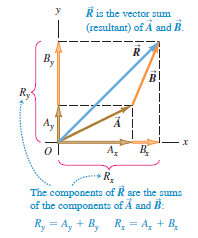
\includegraphics[width=0.3\linewidth]{ch1img17.png}
\end{center}
\end{enumerate}

We discussed vectors that lie in the xy-plane only, but the component method works just as well for vectors having any direction in space. We can introduce a z-axis perpendicular to the xy-plane; then in general a vector $\overrightarrow{A}$  has components $A_x$, $A_y$, $A_z$ in the three coordinate directions with its magnitude $A$ as\\\\
\centerline{$A = \sqrt{{A_x}^2 + {A_y}^2 + {A_z}^2}$}

\begin{examplebox}
\textbf{Example 1.7} \textit{Using components to add vectors.}

Three players on a reality TV show are brought to the center of a large, flat field. Each is given a meter stick, a compass, a calculator, a shovel, and (in a different order for each contestant) the following three displacements:\\

$\overrightarrow{A}$: 72.4 m, $32.0^\circ$ east of north.\\
$\overrightarrow{B}$: 57.3 m, $36.0^\circ$ south of west.\\
$\overrightarrow{C}$: 17.8 m due south.\\

The three displacements lead to the point in the field where the keys to a new Porsche are buried. Two players start measuring immediately, but the winner first \textit{calculates} where to go. What does she calculate?

\begin{center}
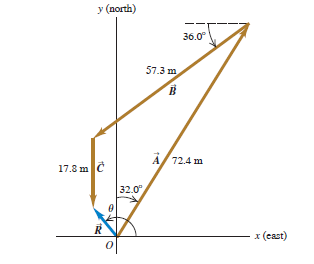
\includegraphics[width=0.4\linewidth]{ch1img19.png}
\end{center}
\begin{mathbox}
\begin{align*}
A_x &= 72.4\, \text{m} \cdot \cos \left(90^\circ - 32\right) = 72.4\, \text{m} \cdot \cos \left(58^\circ\right) = 38.37\,\text{m}\\
A_y &= 72.4\, \text{m} \cdot \sin \left(90^\circ - 32\right) = 72.4\, \text{m} \cdot \sin \left(58^\circ\right) = 61.40\,\text{m}\\\\
B_x &= 57.3\, \text{m} \cdot \cos \left(180^\circ + 36\right) = 57.3\, \text{m} \cdot \cos \left(216^\circ\right) = -46.36\,\text{m}\\
B_y &= 57.3\, \text{m} \cdot \sin \left(180^\circ + 36\right) = 57.3\, \text{m} \cdot \sin \left(216^\circ\right) = -33.68\,\text{m}\\\\
C_x &= 17.8\, \text{m} \cdot \cos \left(270^\circ\right) = 0.00\,\text{m}\\
C_y &= 17.8\, \text{m} \cdot \sin \left(270^\circ\right) = -17.80\,\text{m}\\\\
R_x &= -7.99\, \text{m} \quad \text{and} \quad R_y = 9.92\, \text{m}\\\\
R &= \sqrt{{-7.99\, \text{m}}^2 + {9.92\, \text{m}}^2} = \underline{12.7\, \text{m}}\\\\
\theta &= \arctan \frac{9.92\, \text{m}}{-7.99 \text{m}} = -51^\circ\\
\theta\,&= 180 + \left(-51\right) = \underline{129^\circ}
\end{align*}
\end{mathbox}
\end{examplebox}

\section{Unit Vectors}
A \textbf{unit vector} is a vector that has a magnitude of 1, with no units. Its only purpose is to \textit{point}, that is, to describe a direction in space. Unit vectors provide a convenient notation for many expressions involving components of vectors. We will always include a caret to distinguish it from ordinary vectors.\\
In an xy-coordinate system, we can define a unit vector $\hat{i}$ that points in the direction of the positive x-axis and a unit vector $\hat{j}$ that points in the direction of the positive y-axis. Then we can write a vector $\overrightarrow{A}$ in terms of its components, such as

\begin{center}
$\overrightarrow{A} = A_x\hat{i} + A_y\hat{j}$ 
\end{center}
\vspace{-10pt}
Using unit vectors, we can express the vector sum $\overrightarrow{R}$ of two vectors $\overrightarrow{A}$ and $\overrightarrow{B}$ as follows (this also applies to \textit{n} dimensional vectors):
\begin{mathbox}
\begin{align*}
\overrightarrow{A} &= \left(A_x \hat{i} + A_y \hat{j}\right) \\ 
\overrightarrow{B} &= \left(B_x \hat{i} + B_y \hat{j}\right) \\
\overrightarrow{R} &= \overrightarrow{A} + \overrightarrow{B} \\
&= \left(A_x\hat{i} + A_y\hat{j} \right) + \left(B_x\hat{i} + B_y\hat{j}\right) \\
&= \left(A_x + B_x\right) \cdot \hat{i} + \left(A_y + B_y\right) \cdot \hat{j} \\
&= R_x \hat{i} + R_y \hat{j}
\end{align*}
\end{mathbox}

\begin{examplebox}
\textbf{Example 1.8} \textit{Using unit vectors.}\\

Given the two displacements\\
$\overrightarrow{D} = \left(6.00\hat{i} + 3.00\hat{j} - 1.00\hat{k}\right) \text{m}$\\
$\overrightarrow{E} = \left(4.00\hat{i} - 5.00\hat{j} + 8.00\hat{k}\right) \text{m}$\\

Find the magnitude of the displacement $2\overrightarrow{D} - \overrightarrow{E}$.

\begin{mathbox}
\begin{align*}
2\overrightarrow{D}\\
&= 2 \left(6.00\hat{i} + 3.00\hat{j} - 1.00\hat{k}\right) \text{m} \\
&= \left(12.00\hat{i} - 6.00\hat{j} + 2.00\hat{k}\right) \text{m}\\\\
\overrightarrow{F} &= {2\overrightarrow{D}} - \overrightarrow{E} \\
&= \left(\left(12.00\hat{i} + 6.00\hat{j} - 2.00\hat{k}\right) - \left(4.00\hat{i} - 5.00\hat{j} + 8.00\hat{k}\right)\right) \text{m} \\
&= \underline{\left(8.00\hat{i} + 11.00\hat{j} - 10.00\hat{k}\right) \text{m}} \\\\
F &= \sqrt{\left(8.00\text{m}\right)^2 + \left(11.00\text{m}\right)^2 - \left(10.00\text{m}\right)^2} \\
&= 16.9\, m
\end{align*}
\end{mathbox}
\end{examplebox}

\begin{tipbox}
By using unit vectors, you can write a single equation for vector addition that incorporates the x-, y-, and z- components.
\end{tipbox}

\section{Products of Vectors}
We observed how vector addition develops naturally from the problem of combining displacements. It will prove useful for calculations with many other vector quantities. We can also express many physical relationships by using \textit{products} of vectors. Vectors are not ordinary numbers, so we can't directly apply ordinary multiplication to vectors. We'll define two different kinds of products of vectors. The first, called the \textit{scalar product}, yields a result that is a scalar quantity. The second, the \textit{vector product} yields another vector.

\subsection*{Scalar Product}
We denote the scalar product of two vectors $\overrightarrow{A}$ and $\overrightarrow{B}$ by $\overrightarrow{A} \cdot \overrightarrow{B}$. Because of this notation, the scalar product is also called the \textbf{dot product}. Although $\overrightarrow{A}$ and $\overrightarrow{B}$ are vectors, the quantity $\overrightarrow{A} \cdot \overrightarrow{B}$ is a \textit{scalar}.

To define the scalar product $\overrightarrow{A} \cdot \overrightarrow{B}$, we draw the two vectors $\overrightarrow{A}$ and $\overrightarrow{B}$ with their tails at the same point. The angle \phi\, between their directions ranges from $0^\circ$ to $180^\circ$. The figure below shows the projection of vector $\overrightarrow{B}$ onto the direction of $\overrightarrow{A}$; this projection is the component of $\overrightarrow{B}$ in the direction of $\overrightarrow{A}$ and is equal to $B\cos\phi$. We define $\overrightarrow{A} \cdot \overrightarrow{B}$ to be the magnitude of $\overrightarrow{A}$ multiplied by the component of $\overrightarrow{B}$ in the direction of $\overrightarrow{A}$.

Alternatively, we can define $\overrightarrow{A} \cdot \overrightarrow{B}$ to be the magnitude of $\overrightarrow{B}$ mulitplied by the component of $\overrightarrow{A}$ in the direction of $\overrightarrow{B}$.

\begin{mathbox}
\begin{align*}
\overrightarrow{A} \cdot \overrightarrow{B} = AB\cos\phi\, = \left| \overrightarrow{A}\right| \left| \overrightarrow{B}\right| \cos\phi\,
\end{align*}
\end{mathbox}

\begin{figure}[ht]
  \centering
  % First minipage for the first image
  \begin{minipage}[b]{0.4\linewidth}
    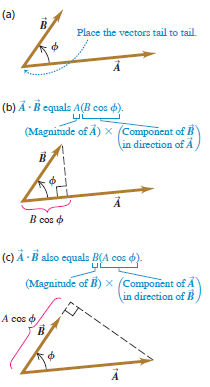
\includegraphics[width=\linewidth]{ch1img20.png}
    \caption{Scalar product for two vectors.}
    \label{fig:image1}
  \end{minipage}
  \hfill % This adds a little space between the two minipages
  % Second minipage for the second image
  \begin{minipage}[b]{0.45\linewidth}
    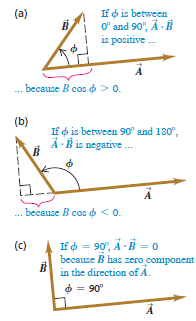
\includegraphics[width=\linewidth]{ch1img21.png}
    \caption{Scalar product can be positive, negative or zero.}
    \label{fig:image2}
  \end{minipage}
\end{figure}

The scalar product is a scalar quantity, not a vector, and may be positive, negative, or zero. When \phi\, is between $0^\circ$ and $90^\circ$, $\cos\phi\, > 0$ and the scalar product is positive. 
When \phi is between $90^\circ$ and $180^\circ$ so $\cos \phi$\,, the component of $\overrightarrow{B}$ in the direction of $\overrightarrow{A}$ is negative, and $\overrightarrow{A} \cdot \overrightarrow{B}$ is negative. Finally when \phi\, is equal to $90^\circ$, $\overrightarrow{A} \cdot \overrightarrow{B} = 0$. \textit{The scalar product of two perpendicular vectors is always zero}.\\
For any two vectors $\overrightarrow{A}$ and $\overrightarrow{B}$, $AB\cos\phi = BA\cos\phi$. This means that $\overrightarrow{A} \cdot \overrightarrow{B} = \overrightarrow{B} \cdot \overrightarrow{A}$. The scalar product obeys the commutative law of multiplication; the order of the two vectors does not matter.\\
We use scalar product to describe work done by a force, calculating electric potential, determine the effects of varying magnetic fields on electric circuits among other things.\\

\subsection*{Using Components to Calculate the Scalar Product}
We can calculate the scalar product $\overrightarrow{A} \cdot \overrightarrow{B}$ directly if we know the x-, y-, and z- components of $\overrightarrow{A}$ and $\overrightarrow{B}$. To see how this is done, let's first work out the scalar products of the unit $\hat{i}$, $\hat{j}$, $\hat{k}$. All unit vectors have magnitude 1 and are perpendicular to each other. Using our definition for the scalar product, we find
\begin{mathbox}
\begin{align*}
\hat{i} \cdot \hat{i} &= \hat{j} \cdot \hat{j} = \hat{k} \cdot \hat{k} = \left(1\right) \left(1\right) \cos 0^\circ = 1\\
\hat{i} \cdot \hat{j} &= \hat{i} \cdot \hat{k} = \hat{j} \cdot \hat{k} = \left(1\right) \left(1\right) \cos 90^\circ = 0
\end{align*}
\end{mathbox}

Now we express $\overrightarrow{A}$ and $\overrightarrow{B}$ in terms of their components, expand the product and use these products of unit vectors.

\begin{mathbox}
\begin{align*}
\overrightarrow{A} \cdot \overrightarrow{B} &= \left(A_x\hat{i} + A_y\hat{j} + A_z\hat{k}\right) \cdot \left(B_x\hat{i} + B_y\hat{j} + B_z\hat{k}\right) \\
&= A_x\hat{i} \cdot B_x\hat{i} + A_x\hat{j} \cdot B_y\hat{j} + A_x\hat{k} \cdot B_z\hat{k}\, +\\
&\hspace{4.5mm} A_y\hat{j} \cdot B_x\hat{i}\, + A_y\hat{j} \cdot B_y\hat{j} + A_y\hat{j} \cdot B_z\hat{k}\, +\\
&\hspace{4.5mm} A_z\hat{k} \cdot B_x\hat{i}\, + A_z\hat{k} \cdot B_y\hat{j} + A_z\hat{k} \cdot B_z\hat{k}\,\\\\
&= A_x B_x\hat{i}\cdot\hat{i} + A_y B_y\hat{i}\cdot\hat{j} + A_x B_z\hat{i}\cdot\hat{k}\, + \\ 
&\hspace{4.5mm} A_y B_x\hat{j} \cdot \hat{i} + A_y B_y\hat{j} \cdot \hat{j} + A_y B_z\hat{j} \cdot \hat{k}\, +\\
&\hspace{4.5mm} A_z B_x\hat{k} \cdot \hat{i} + A_z B_y\hat{k} \cdot \hat{j} + A_z B_z\hat{k} \cdot \hat{k} \\\\
&\hspace{4.5mm} \underline{\overrightarrow{A} \cdot \overrightarrow{B} = A_x B_x + A_y B_y + A_z B_z}
\end{align*}
\end{mathbox}
 
Thus the \textit{scalar product of two vectors is the sum of the products of their respective components}.\\

The scalar product gives a straightforward way to find the angle \phi\, between any two vectors $\overrightarrow{A}$ and $\overrightarrow{B}$ whose components are known. We can use this equation to find the scalar product of $\overrightarrow{A}$ and $\overrightarrow{B}$.

\begin{examplebox}
\textbf{Example 1.9} \textit{Calculating a scalar product.}\\

Find the scalar product $\overrightarrow{A}$ \cdot $\overrightarrow{B}$ of the two vectors in the fig. below. The magnitudes of the vectors are $A = 4.00$ and $B = 5.00$.

\begin{center}
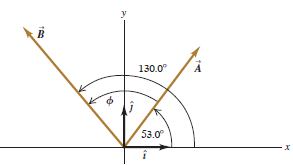
\includegraphics[width=0.5\linewidth]{ch1img22.png}
\end{center}
\begin{mathbox}
\begin{align*}
&= \overrightarrow{A} \cdot \overrightarrow{B}\\ 
&= A B \cos \phi\\
&= \left(4.00\right)\left(5.00\right) \cos\left(130 - 53\right)^\circ\\
&= \left(4.00\right)\left(5.00\right) \cos\left(77\right)^\circ\\
&= 4.50
\end{align*}
\end{mathbox}
\end{examplebox} 

\begin{examplebox}
\textbf{Example 1.10} \textit{Finding an angle with the scalar product.}\\

Find the angle between the vectors\\
$\overrightarrow{A} = 2.00\hat{i} + 3.00\hat{j} + 1.00\hat{k}$ \quad and \quad $\overrightarrow{B} = -4.00\hat{i} + 2.00\hat{j} - 1.00\hat{k}$\\
\begin{center}
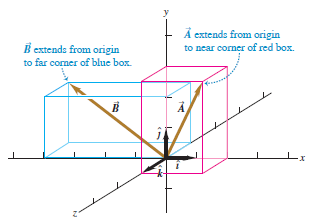
\includegraphics[width=0.5\linewidth]{ch1img23.png}
\end{center}
\begin{mathbox}
\begin{align*}
\overrightarrow{A} \cdot \overrightarrow{B} &= A B \cos \phi\ \\
\cos \phi &= \frac{\overrightarrow{A} \cdot \overrightarrow{B}}{A B}\\\\
\overrightarrow{A} \cdot \overrightarrow{B} &= A_xB_x + A_yB_y + A_zB_z\\
&= \left(2.00\right) \left(-4.00\right) + \left(3.00\right) \left(2.00\right) + \left(1.00\right) \left(-1.00\right)\\
&= -3.00\\\\
A B\\ 
A &= \sqrt{\left(2.00\right)^2 + \left(3.00\right)^2 + \left(1.00\right)^2} = \sqrt{14}\\
B &= \sqrt{\left(-4.00\right)^2 + \left(2.00\right)^2 + \left(-1.00\right)^2} = \sqrt{21.00}\\\\
\cos \phi &= \frac{-3.00}{\sqrt{14.00} \sqrt{21.00}} = -0.175\\\\
&\underline{\phi = 100^\circ}
\end{align*}
\end{mathbox}
\end{examplebox} 
\begin{tipbox}
We can find the angle \phi\, between two vectors $\overrightarrow{A}$ and $\overrightarrow{B}$ whose components are known by first finding their scalar product and then using the equation $\overrightarrow{A} \cdot \overrightarrow{B} = AB \cos \phi$.
\end{tipbox}

\subsection*{Vector Products}
We denote the \textbf{vector product} of two vectors $\overrightarrow{A}$ and $\overrightarrow{B}$, also called the \textbf{cross product}, by $\overrightarrow{A} \times \overrightarrow{B}$. As the name indicates, this is a vector. 
\begin{tipbox}
We use vector products among other things, to describe torque, angular momentum, magnetic fields, and forces.
\end{tipbox}
To define the vector product  $\overrightarrow{A} \times \overrightarrow{B}$, we again draw the vectors  $\overrightarrow{A}$ and $\overrightarrow{B}$ with their tails at the same point. The two vectors then lie in a plane. We define the vector product to be a vector quantity with a direction perpendicular to this plane and a magnitude equal to $AB\sin\phi$. That is, if $\overrightarrow{C} = \overrightarrow{A} \times \overrightarrow{B}$, then
\begin{mathbox}
\begin{align*}
C = A B \sin \phi
\end{align*}
\end{mathbox}
There are always two directions perpendicular to a given plane, one on each side of the plane. We choose which of these is the direction of $\overrightarrow{A} \times \overrightarrow{B}$ as follows. Imagine rotating $\overrightarrow{A}$ about the perpendicular line until $\overrightarrow{A}$ is aligned with $\overrightarrow{B}$ , choosing the smaller of the two possible angles between $\overrightarrow{A}$ and $\overrightarrow{B}$ . Curl the fingers of your right hand around the perpendicular line so that your fingertips point in the direction of rotation; your thumb will then point in the direction of $\overrightarrow{A} \times \overrightarrow{B}$.

Similarly, we determine the direction of $\overrightarrow{B} \times \overrightarrow{A}$ by rotating $\overrightarrow{B}$ onto $\overrightarrow{A}$. The result is a vector that is \textit{opposite} to the vector $\overrightarrow{A} \times \overrightarrow{B}$. The vector product is \textit{not} commutative, instead is \textbf{anticommutative}: For any two vectors $\overrightarrow{A}$ and $\overrightarrow{B}$:
\begin{mathbox}
\begin{align*}
\overrightarrow{A} \times \overrightarrow{B} = - \overrightarrow{B} \times \overrightarrow{A}
\end{align*}
\end{mathbox}

\subsection*{Using Components to Calculate the Vector Product}
If we know the components of $\overrightarrow{A}$ and $\overrightarrow{B}$, we can calculate the components of vector product by using a procedure similar to that for the scalar product. First we work out the multiplication table for unit vectors $\hat{i}$, $\hat{j}$, and $\hat{k}$, all three of which are perpendicular to each other. The vector product of any vector with respect to itself is zero, so
\begin{mathbox}
\begin{align*}
\hat{i} \times \hat{i} &= \hat{j} \times \hat{j} = \hat{k} \times \hat{k} = 0\\\\
\hat{i} \times \hat{j} &= - \hat{j} \times \hat{i} = \hat{k}\\
\hat{j} \times \hat{k} &= - \hat{k} \times \hat{j} = \hat{i}\\
\hat{k} \times \hat{i} &= -\hat{i} \times \hat{k} = \hat{j}
\end{align*}
\end{mathbox}
 
Next we express $\overrightarrow{A}$ and $\overrightarrow{B}$ in terms of their components and the corresponding unit vectors, we get:
\begin{mathbox}
\begin{align*}
\overrightarrow{A} \times \overrightarrow{B} = \left(A_yB_z - A_zB_y\right)\hat{i}\, + \left(A_zB_x - A_xBz\right)\hat{j}\, + \left(A_xB_y - A_yB_x\right)\hat{k}\,
\end{align*}
\end{mathbox}

\pagebreak

\section{Exercises}

\begin{legendbox}
\textbf{Difficulty Levels:} +, ++, +++\\
\textbf{CP}: Cumulative Problems \qquad \textbf{CALC}: Calculus Problems\\
\textbf{DATA}: Problems involving real data, scientific evidence, experimental design, and/or statistical reasoning.\\
\textbf{BIO}: Biosciences problems.
\end{legendbox}

\begin{examplebox}
\textbf{Exercise 1.1 [+]}\\
Starting with the definition $1$ in. $= 2.54$ cm, find the number of: \\
a) kilometers in $1.00$ mile. \qquad b) feet in $1.00$ km.
\begin{mathbox}
\begin{align*}
\text{a) kilometers in 1.00 mile.}\\
1.00\, \text{mi.} &= 5280\, \text{ft.}\\\\
1.00\, \text{ft.} &= 12\, \text{in.}\\
1.00\, \text{mi.} &= 5280\, \cancel{\text{ft.}} \cdot \frac{12\, \text{in.}}{1\, \cancel{\text{ft.}}} = 63360\, \text{in.}\\\\
1.00\, \text{mi.} &= 63360\, \text{in.} = 63360\, \cancel{\text{in.}} \times \frac{2.54\, \text{cm.}}{1.00\, \cancel{\text{in.}}} = 160934.4\, \text{cm.}\\\\
&= 160934.4\, \cancel{\text{cm.}} \cdot \frac{0.01\, \cancel{\text{m.}}}{1.00\, \cancel{\text{cm.}}} \cdot \frac{0.0001\, \text{km.}}{1.00\, \cancel{\text{m}}}\\
&= \underline{1.61\, \text{km.}}\\\\
\text{b) feet in 1.00 km.}\\
&= 1.00\, \cancel{\text{km.}} \cdot \frac{1\, \text{mi.}}{1.61\, \cancel{\text{km}}}\\
&= 0.6211180\, \cancel{\text{mi.}} \cdot \frac{5280\, \text{ft.}}{1.00\, \cancel{\text{mi.}}}\\
&= \underline{3281\, \text{ft.}}
\end{align*}
\end{mathbox}
\end{examplebox} 

\begin{examplebox}
\textbf{Exercise 1.2 [++]}\\
According to the label on a bottle of salad dressing, the volume of the contents is $0.473$ liter (L). Using only the conversions $1$ L = ${1000\, \text{cm}}^3$ and $1$ in. = $2.54$ cm, express this volume in cubic inches.
\begin{mathbox}
\begin{align*}
&= 0.473\, \text{L} \cdot \frac{1000\, \text{cm}^3}{1.00\, \text{L}}\\
&= 473\, \text{cm}^3 \cdot \frac{1.00\, \text{in}^3}{2.54\, \text{cm}^3}\\
&= \underline{28.87\, \text{in.}^3}
\end{align*}
\end{mathbox}
\end{examplebox} 

\begin{examplebox}
\textbf{Exercise 1.3 [++]}\\
How many nanoseconds does it take light to travel $1.00$ ft. in vacuum? (This result is a useful quantity to remember.)
\begin{mathbox}
\begin{align*}
&= 1\, \text{ft.} \cdot \frac{30.48\, \text{cm.}}{1.00\, \text{ft.}} \cdot \frac{1.00\, \text{m}}{100\, \text{cm}} = 0.3048\, \text{m}\\
&= 2.99792458 
\end{align*}
\end{mathbox}
\end{examplebox} 